% main.tex - Solutions to the ES202 term assignment
% Copyright (C) 2026  Emir Baha YILDIRIM
%
% This program is free software: you can redistribute it and/or modify
% it under the terms of the GNU General Public License as published by
% the Free Software Foundation, either version 3 of the License, or
% (at your option) any later version.
%
% This program is distributed in the hope that it will be useful,
% but WITHOUT ANY WARRANTY; without even the implied warranty of
% MERCHANTABILITY or FITNESS FOR A PARTICULAR PURPOSE.  See the
% GNU General Public License for more details.
%
% You should have received a copy of the GNU General Public License
% along with this program.  If not, see <https://www.gnu.org/licenses/>.
\documentclass{article}
\usepackage{amsmath, amssymb, physics, hyperref, tikz}
\author{Emir Baha Yıldırım\\ID: 2675619}
\title{ES202 - Assignment Solutions}
\date{05/01/2026}
\hypersetup{
    colorlinks=true,
    linkcolor=blue,
    filecolor=magenta,      
    urlcolor=cyan,
    }
\begin{document}
\maketitle

\pagebreak

\tableofcontents

\pagebreak

\section{Introduction}

% I hope the instructor allows us to use LaTeX, I really don't want to write
% this shit out.

These are my solutions to the assignment given in the course ES202.
\\
\subsection{AI Policy of This Paper}
Large-Language-Model's (LLM) are only used in the formatting of this file. At no
point, LLM's are used to solve the questions in the assignment, unlike other
students taking the course who like to ask the help of LLMs even during the
examinations. The reason this is written in LaTeX rather than by hand, is only
because I have no time to do it by hand, and wanted to improve my LaTeX skills.
The git commit history can be found in the GitHub repository \\
\href{https://github.com/jayshozie/es202-assignment}{jayshozie/es202-assignment},
also as a proof of the fact that this entire document was written by hand.
\pagebreak

% Question 1

\section{Question 1}
\label{question-1}
\textbf{Problem}
An airplane is monitored at coordinates $(5, 7, 4)$ relative to the airport
(South, East, Up). Find the directional angles of the plane.
\\
\\
\textbf{Solution:}
Let the position vector of the plane be $\vec{r}$. We define the axes such that
$x=\text{South}$, $y=\text{East}$, and $z=\text{Up}$.
\begin{align*}
	% define the vector of the airplane
	\vec{r}         & = 5\hat{i} + 7\hat{j} + 4\hat{k} \\
	\norm*{\vec{r}} & = \sqrt{5^{2} + 7^{2} + 4^{2}}   \\
	                & = \sqrt{25 + 49 + 16}            \\
	                & = \sqrt{90}                      \\
	                & \approx 9.4868                   \\
\end{align*}
The directional angles $\alpha, \beta, \gamma$ are given by the direction
cosines:
\begin{alignat*}{3}
	% Row 1: Symbolic Formulas
	\alpha & = \cos^{-1}\left(\frac{r_{x}}{\norm*{\vec{r}}}\right) \quad &
	\beta  & = \cos^{-1}\left(\frac{r_{y}}{\norm*{\vec{r}}}\right) \quad &
	\gamma & = \cos^{-1}\left(\frac{r_{z}}{\norm*{\vec{r}}}\right)         \\
	% Row 2: Numerical Substitution (Empty LHS aligns to the equals sign above)
	       & = \cos^{-1}\left(\frac{5}{\sqrt{90}}\right)                 &
	       & = \cos^{-1}\left(\frac{7}{\sqrt{90}}\right)                 &
	       & = \cos^{-1}\left(\frac{4}{\sqrt{90}}\right)                   \\
	% Row 3: Final Answer
	       & \approx 58.19^\circ                                         &
	       & \approx 42.45^\circ                                         &
	       & \approx 64.06^\circ
\end{alignat*}
\pagebreak

% Question 2

\section{Question 2}
\label{question-2}
\textbf{Problem}
Prove that $\norm*{\vec{a}\cdot\vec{b}} \le \norm*{\vec{a}}\cdot\norm*{\vec{b}}$
\\
\\
\textbf{Solution}
By the geometric definition of the dot product, the angle $\theta$ between the
vectors $\norm*{\vec{a}}$ and $\norm*{\vec{b}}$ is given by:
\begin{align*}
	\vec{a} \cdot \vec{b} & = \norm*{\vec{a}} \norm*{\vec{b}} \cos{\theta} \\
\end{align*}
We know that for any real angle $\theta$, the cosine function is bounded:
\begin{align*}
	-1 \le \cos{\theta} \le 1 \implies \norm*{\cos{\theta}} \le 1
\end{align*}
Substituting this inequality back into our original equation:
\begin{align}
	\nonumber \norm*{\vec{a} \cdot \vec{b}} & = \norm*{\vec{a}} \cdot \norm*{\vec{b}} \underbrace{\norm*{\cos{\theta}}}_{\le 1}
	\nonumber \intertext{Therefore proving:}
	\norm*{\vec{a} \cdot \vec{b}}           & \le \norm*{\vec{a}}\cdot\norm*{\vec{b}} \label{cauchy-schwartz}
\end{align}
\pagebreak

% Question 3

\section{Question 3}
\label{question-3}
\textbf{Problem}
Prove $\norm*{\vec{a} + \vec{b}} \le \norm*{\vec{a}} + \norm*{\vec{b}}$
\\
\\
\textbf{Solution}
Since magnitudes are non-negative by definition, proving the inequality is
equivalent to proving it for the squares of the magnitudes. Consider the square
of the sum:
\begin{align*}
	\norm*{\vec{a} + \vec{b}}^{2} & = (\vec{a} + \vec{b}) \cdot (\vec{a} + \vec{b})                            \\
	                              & = \vec{a} \cdot \vec{a} + 2(\vec{a} \cdot \vec{b}) + \vec{b} \cdot \vec{b} \\
	                              & = \norm*{\vec{a}}^{2} + 2(\vec{a} \cdot \vec{b}) + \norm*{\vec{b}}^{2}     \\
\end{align*}
From (\ref{cauchy-schwartz})
(\href{https://en.wikipedia.org/wiki/Cauchy%E2%80%93Schwarz_inequality}{Cauchy-Schwartz Inequality}),
we established that
\begin{align*}
	\vec{a} \cdot \vec{b} \le \norm*{\vec{a} \cdot \vec{b}} \le \norm*{\vec{a}}\norm*{\vec{b}}
\end{align*}
We substitute this upper bound into the equation:
\begin{align*}
	\norm*{\vec{a} + \vec{b}}^2 & \le \norm*{\vec{a}}^2 + 2\norm*{\vec{a}}\norm*{\vec{b}} + \norm*{\vec{b}}^2 \\
	\intertext{Recognizing the right-hand side as a perfect expansion $(x+y)^{2}=x^{2} + 2xy + y^{2}$:}
	\norm*{\vec{a} + \vec{b}}^2 & \le \left( \norm*{\vec{a}} + \norm*{\vec{b}} \right)^2
\end{align*}
Taking the square root of both sides, which is valid since magnitudes are
non-negative:
\begin{align}
	\norm*{\vec{a} + \vec{b}} \le \norm*{\vec{a}} + \norm*{\vec{b}} \label{triangle-inequality}
\end{align}

\pagebreak

% Question 4

\section{Question 4}
\textbf{Problem}
Prove $\norm*{\vec{a} \times \vec{b}}^{2} = \norm*{\vec{a}}^{2}\norm*{\vec{b}}^{2} - (\vec{a}\cdot\vec{b})^{2}$
\\
\\
\textbf{Solution}
Magnitude of the vector-product of two vectors $\vec{a}$ and $\vec{b}$,
separated by an angle $\theta$, is defined as:
\begin{align}
	\norm*{\vec{a} \times \vec{b}}                                     & = \norm*{\vec{a}} \norm*{\vec{b}} \sin{\theta} \label{cross-vector-product-magnitude-definition}     \\
	\nonumber \intertext{Square both sides:}
	\nonumber \norm*{\vec{a} \times \vec{b}}^{2}                       & = (\norm*{\vec{a}} \norm*{\vec{b}} \sin{\theta})^{2}                                                 \\
	\nonumber                                                          & = \norm*{\vec{a}}^{2} \norm*{\vec{b}}^{2} \sin^{2}{\theta}
	\nonumber \intertext{Since,}
	\nonumber \cos^{2}{\theta} + \sin^{2}{\theta}                      & = 1                                                                                                  \\
	\nonumber \sin^{2}{\theta}                                         & = 1 - \cos^{2}{\theta}
	\nonumber \intertext{By substituting that to our original equality's right-hand side, we get:}
	\nonumber \norm*{\vec{a} \times \vec{b}}^{2}                       & = \norm*{\vec{a}}^{2} \norm*{\vec{b}}^{2} (1 - \cos^{2}{\theta})
	\nonumber \intertext{Then, by distributing $\norm*{\vec{a}}^{2} \norm*{\vec{b}}^{2}$, we get:}
	\nonumber                                                          & = \norm*{\vec{a}}^{2} \norm*{\vec{b}}^{2} - \norm*{\vec{a}}^{2} \norm*{\vec{b}}^{2} \cos^{2}{\theta}
	\nonumber \intertext{Observe that,}
	\nonumber \norm*{\vec{a}}^{2} \norm*{\vec{b}}^{2} \cos^{2}{\theta} & = (\norm*{\vec{a}}\norm*{\vec{b}}\sin{\theta})^{2} = (\vec{a} \cdot \vec{b})^{2}
	\nonumber \intertext{Thus, by substituting that, we complete our proof:}
	\norm*{\vec{a} \times \vec{b}}^{2}                                 & = \norm*{\vec{a}}^{2} \norm*{\vec{b}}^{2} - (\vec{a} \cdot \vec{b})^{2}
\end{align}

\pagebreak

% Question 5

\section{Question 5}
\textbf{Problem}
Let vectors $\vec{u}_{1} = (1,0,0)$, $\vec{u}_{2} = (1,1,0)$, and
$\vec{u}_{3} = (1,1,1)$ form a basis for the vector space $\mathbb{R}^{3}$. Show
that these vectors are linearly independent and express vector
$\vec{a} = (3,-4,8)$ as a linear combination of them.
\\
\\
\textbf{Solution}
We will divide our solution to two parts. In the first part, we'll prove that
the given vectors $\vec{u}_{1}$, $\vec{u}_{2}$, and $\vec{u}_{3}$ are linearly
independent, thus forming a basis for $\mathbb{R}^{3}$; then we'll find a linear
combination for the vector $\vec{a}$.
\\
\\
\textbf{Part 1: Linear Independence}
We form a matrix $A$ with the vectors $\vec{u}_{1}$, $\vec{u}_{2}$, and
$\vec{u}_{3}$ as columns. The vectors are linearly independent if
$\det(A) \neq 0$.
\begin{align*}
	\det(A) =
	\begin{vmatrix}
		1 & 1 & 1 \\
		0 & 1 & 1 \\
		0 & 0 & 1
	\end{vmatrix}
\end{align*}
Since this is an upper-triangular matrix, the determinant is the product of the
diagonal entries:
\begin{align*}
	\det(A) = 1 \cdot 1 \cdot 1 = 1 \neq 0
\end{align*}
Therefore, the vectors are linearly independent and form a basis for
$\mathbb{R}^3$.
\\
\\
\textbf{Part 2: Linear Combination}
We wish to find coefficients $c_{1}$, $c_{2}$, and $c_{3}$ such that:
\begin{align*}
	c_{1}\cdot\vec{u}_{1} + c_{2}\cdot\vec{u}_{2} + c_{3}\cdot\vec{u}_{3} = \vec{a}
\end{align*}
This corresponds to the linear system:
\begin{align*}
	\left[
		\begin{array}{ccc|c}
			1 & 1 & 1 & 3  \\
			0 & 1 & 1 & -4 \\
			0 & 0 & 1 & 8  \\
		\end{array}
		\right]
\end{align*}

Using back-substitution:
\begin{align*}
	1. \quad & c_{3} = 8                                                       \\
	2. \quad & c_{2} + 8 = -4 \implies c_{2} = -12                             \\
	3. \quad & c_{1} + (-12) + 8 = 3 \implies c_{1} - 4 = 3 \implies c_{1} = 7
\end{align*}

Using those coefficients, we can say that:
\begin{align*}
	\vec{a} = 7\vec{u}_{1} - 12\vec{u}_{2} + 8\vec{u}_{3}
\end{align*}

\pagebreak

% Question 6

\section{Question 6}

\textbf{Problem}
Obtain an orthonormal set from the given set of vectors using Gram-Schmidt
Orthogonalization Process:
\begin{align*}
	\vec{B} =
	\left\{
	\left(
	\frac{1}{2}, \frac{1}{2}, 1
	\right)
	\left(
	-1, 1, -\frac{1}{2}
	\right)
	\left(
	-1, \frac{1}{2}, 1
	\right)
	\right\}
\end{align*}
\\
\\
\textbf{Solution}
Let the given vectors be $\vec{v}_{1}$, $\vec{v}_{2}$, and $\vec{v}_{3}$. We
will generate an orthogonal set $\{\vec{u}_{1}, \vec{u}_{2}, \vec{u}_{3}\}$ and
then normalize them to get the orthonormal set
$\{\vec{e}_{1}, \vec{e}_{2}, \vec{e}_{3}\}$.
\\
\\
\textbf{Step 1. Process the first vector}
To use the Gram-Schmidt Orthogonalization Process, we need to pick a vector. For
convention, we'll pick $\vec{v}_{1}$ as our first vector.
\begin{align*}
	\vec{u}_{1}       & = \vec{v}_{1} = \left(\frac{1}{2}, \frac{1}{2}, 1\right)
	\intertext{Calculating the magnitude of $\vec{u}_{1}$ gives us:}
	\norm*{\vec{u}_1} & = \sqrt{\left(\frac{1}{2}\right)^2 + \left(\frac{1}{2}\right)^2 + 1^2} \\
	                  & = \sqrt{\frac{3}{2}}
	\intertext{So, our first orthonormal vector $\vec{e}_{1}$ is:}
	\vec{e}_{1}       & = \frac{\vec{u}_{1}}{\norm*{\vec{u}_{1}}}                              \\
	                  & = \sqrt{\frac{2}{3}}\left(\frac{1}{2}, \frac{1}{2}, 1\right)
\end{align*}
\textbf{Step 2. Orthogonalize the second vector}
We calculate the projection of $\vec{u}_{2}$ onto $\vec{u}_{1}$.
\begin{align*}
	\vec{v}_{2} \cdot \vec{u}_{1} & = (-1)\left(\frac{1}{2}\right) + (1)\left(\frac{1}{2}\right) + \left(-\frac{1}{2}\right)(1) = -\frac{1}{2} \\
	\vec{u}_{2}                   & = \vec{v}_{2} - \frac{\vec{v}_{2} \cdot \vec{u}_{1}}{\norm*{\vec{u}_{1}}^2} \vec{u}_{1}
	= \left(-1, 1, -\frac{1}{2}\right) - \frac{-1/2}{3/2} \left(\frac{1}{2}, \frac{1}{2}, 1\right)                                             \\
	                              & = \left(-1, 1, -\frac{1}{2}\right) + \frac{1}{3} \left(\frac{1}{2}, \frac{1}{2}, 1\right)
	= \left(-\frac{5}{6}, \frac{7}{6}, -\frac{1}{6}\right)
\end{align*}
We, then, normalize $\vec{u}_{2}$ by:
\begin{align*}
	\norm*{\vec{u}_{2}}^2 & = \frac{25}{36} + \frac{49}{36} + \frac{1}{36} = \frac{75}{36} = \frac{25}{12} \implies \norm*{\vec{u}_{2}} = \frac{5}{2\sqrt{3}}                                                                  \\
	\vec{e}_{2}           & = \frac{\vec{u}_{2}}{\norm*{\vec{u}_{2}}} = \frac{2\sqrt{3}}{5}\left(-\frac{5}{6}, \frac{7}{6}, -\frac{1}{6}\right) = \left(-\frac{\sqrt{3}}{3}, \frac{7\sqrt{3}}{15}, -\frac{\sqrt{3}}{15}\right)
\end{align*}
\\
\textbf{Step 3: Orthogonalize the third vector}
Formula: $\vec{u}_{3} = \vec{v}_{3} - \text{proj}_{\vec{u}_{1}}(\vec{v}_{3}) - \text{proj}_{\vec{u}_{2}}(\vec{v}_{3})$.
First, we compute the projection coefficients:
\begin{align*}
	\frac{\vec{v}_{3} \cdot \vec{u}_{1}}{\norm*{\vec{u}_{1}}^2} & = \frac{(-1)(\frac{1}{2}) + (\frac{1}{2})(\frac{1}{2}) + (1)(1)}{3/2} = \frac{3/4}{3/2} = \frac{1}{2}                                                                             \\
	\frac{\vec{v}_{3} \cdot \vec{u}_{2}}{\norm*{\vec{u}_{2}}^2} & = \frac{(-1)(-\frac{5}{6}) + (\frac{1}{2})(\frac{7}{6}) + (1)(-\frac{1}{6})}{25/12} = \frac{\frac{5}{6} + \frac{7}{12} - \frac{2}{12}}{25/12} = \frac{15/12}{25/12} = \frac{3}{5}
\end{align*}
Now substitute back to find $\vec{u}_{3}$:
\begin{align*}
	\vec{u}_{3} & = \vec{v}_{3} - \frac{1}{2}\vec{u}_{1} - \frac{3}{5}\vec{u}_{2}                                                                                 \\
	            & = \left(-1, \frac{1}{2}, 1\right) - \left(\frac{1}{4}, \frac{1}{4}, \frac{1}{2}\right) - \left(-\frac{1}{2}, \frac{7}{10}, -\frac{1}{10}\right) \\
	            & = \left( -1 - 0.25 + 0.5, \quad 0.5 - 0.25 - 0.7, \quad 1 - 0.5 + 0.1 \right)                                                                   \\
	            & = \left( -0.75, -0.45, 0.6 \right) = \left( -\frac{3}{4}, -\frac{9}{20}, \frac{3}{5} \right)
\end{align*}
Normalize $\vec{u}_{3}$:
\begin{align*}
	\norm*{\vec{u}_{3}}^2 & = \frac{9}{16} + \frac{81}{400} + \frac{9}{25} = \frac{225 + 81 + 144}{400} = \frac{450}{400} = \frac{9}{8}    \\
	\vec{e}_{3}           & = \frac{\vec{u}_{3}}{\sqrt{9/8}} = \frac{2\sqrt{2}}{3} \left( -\frac{3}{4}, -\frac{9}{20}, \frac{3}{5} \right)
	= \left( -\frac{\sqrt{2}}{2}, -\frac{3\sqrt{2}}{10}, \frac{2\sqrt{2}}{5} \right)
\end{align*}

\textbf{Final Answer:} The orthonormal set is
$\{ \vec{e}_{1}, \vec{e}_{2}, \vec{e}_{3} \}$, where:
\begin{align*}
	\vec{e}_{1} & =
	\left(
	\frac{\sqrt{2}}{2\sqrt{3}}, \frac{\sqrt{2}}{2\sqrt{3}}, \frac{\sqrt{2}}{\sqrt{3}}
	\right)         \\
	\vec{e}_{2} & =
	\left(
	-\frac{\sqrt{3}}{3}, \frac{7\sqrt{3}}{15}, -\frac{\sqrt{3}}{15}
	\right)         \\
	\vec{e}_{3} & =
	\left(
	-\frac{\sqrt{2}}{2}, -\frac{3\sqrt{2}}{10}, \frac{2\sqrt{2}}{5}
	\right)
\end{align*}

\pagebreak

% Question 7

\section{Question 7}
\textbf{Problem}
Verify that the matrix $A$ satisfies its own characteristic equation
\[
	A =
	\begin{bmatrix}
		1 & -2 \\
		4 & 5  \\
	\end{bmatrix}
\]
\\
\\
\textbf{Solution}
\\
\textbf{Step 1. Find the Characteristic Equation}
The characteristic equation of a matrix is given by $\det(A - \lambda I) = 0$.
\begin{align*}
	\det(A - \lambda I) & = \begin{vmatrix} 1 - \lambda & -2 \\ 4 & 5 - \lambda \end{vmatrix} \\
	                    & = (1 - \lambda)(5 - \lambda) - (-2)(4)                              \\
	                    & = (5 - \lambda - 5\lambda + \lambda^2) - (-8)                       \\
	                    & = \lambda^2 - 6\lambda + 5 + 8                                      \\
	                    & = \lambda^2 - 6\lambda + 13
\end{align*}
Thus, the characteristic equation is $\lambda^2 - 6\lambda + 13 = 0$.
\\
\textbf{Step 2. Verify for Matrix A}
According to the Cayley-Hamilton theorem, the matrix $A$ should satisfy:
\[
	A^2 - 6A + 13I = 0
\]
First, we calculate $A^2$:
\begin{align*}
	A^2 & = \begin{bmatrix} 1 & -2 \\ 4 & 5 \end{bmatrix} \begin{bmatrix} 1 & -2 \\ 4 & 5 \end{bmatrix} \\
	    & = \begin{bmatrix}
		        (1)(1) + (-2)(4) & (1)(-2) + (-2)(5) \\
		        (4)(1) + (5)(4)  & (4)(-2) + (5)(5)
	        \end{bmatrix}                                                        \\
	    & = \begin{bmatrix}
		        1 - 8  & -2 - 10 \\
		        4 + 20 & -8 + 25
	        \end{bmatrix}
	= \begin{bmatrix} -7 & -12 \\ 24 & 17 \end{bmatrix}
\end{align*}
Now, we substitute $A^2$ and $A$ into the equation:
\begin{align*}
	A^2 - 6A + 13I & = \begin{bmatrix} -7 & -12 \\ 24 & 17 \end{bmatrix} - 6\begin{bmatrix} 1 & -2 \\ 4 & 5 \end{bmatrix} + 13\begin{bmatrix} 1 & 0 \\ 0 & 1 \end{bmatrix}   \\
	               & = \begin{bmatrix} -7 & -12 \\ 24 & 17 \end{bmatrix} - \begin{bmatrix} 6 & -12 \\ 24 & 30 \end{bmatrix} + \begin{bmatrix} 13 & 0 \\ 0 & 13 \end{bmatrix} \\
	               & = \begin{bmatrix}
		                   -7 - 6 + 13 & -12 - (-12) + 0 \\
		                   24 - 24 + 0 & 17 - 30 + 13
	                   \end{bmatrix}                                                                                                                         \\
	               & = \begin{bmatrix} 0 & 0 \\ 0 & 0 \end{bmatrix}
\end{align*}
The result is the zero matrix, verifying that $A$ satisfies its own characteristic equation.

\pagebreak

% Question 8

\section{Question 8}
\textbf{Problem}
Compute
$
	A^{m}:
	A = \begin{bmatrix}
		-1 & 2  \\
		0  & -3 \\
	\end{bmatrix}
$, $m = 6$.
\\
\\
\textbf{Solution}
We will compute $A^6$ by diagonalizing the matrix.
We find matrices $P$ and $D$ such that $A = PDP^{-1}$, which implies $A^6 = PD^6P^{-1}$.
\\
\\
\textbf{Step 1. Find Eigenvalues}
Since $A$ is an upper triangular matrix, its eigenvalues are the diagonal entries:
\[
	\lambda_{1} = -1, \quad \lambda_{2} = -3
\]
\\
\\
\textbf{Step 2. Find Eigenvectors}
\\
\\
For $\lambda_{1} = -1$:
\[
	(A - (-1)I)\vec{v}_{1} = \begin{bmatrix} 0 & 2 \\ 0 & -2 \end{bmatrix} \begin{bmatrix} x \\ y \end{bmatrix} = \begin{bmatrix} 0 \\ 0 \end{bmatrix}
\]
From row 1:
\begin{align*}
	2y = 0 \implies y=0
\end{align*}
$x$ is a free variable, so we choose
\begin{align*}
	\vec{v}_{1} =
	\begin{bmatrix}
		1 \\
		0
	\end{bmatrix}
\end{align*}
\\
For $\lambda_{2} = -3$:
\[
	(A - (-3)I)\vec{v}_{2} = \begin{bmatrix} 2 & 2 \\ 0 & 0 \end{bmatrix} \begin{bmatrix} x \\ y \end{bmatrix} = \begin{bmatrix} 0 \\ 0 \end{bmatrix}
\]
From row 1:
\begin{align*}
	2x + 2y = 0 \implies x = -y
\end{align*}
Let $y=1$, then $x=-1$. We choose
\begin{align*}
	\vec{v}_{2} =
	\begin{bmatrix}
		-1 \\
		1
	\end{bmatrix}
\end{align*}
\\
\\
\textbf{Step 3: Construct Matrices $P$ and $D$}
The matrix $P$ consists of the eigenvectors, and $D$ contains the eigenvalues:
\[
	P = \begin{bmatrix} 1 & -1 \\ 0 & 1 \end{bmatrix}, \quad D = \begin{bmatrix} -1 & 0 \\ 0 & -3 \end{bmatrix}
\]
We need to find to have the final diagonalization formula $P^{-1}$. Observe that
the determinant of $P$ is $(1)(1) - (-1)(0) = 1$.
\[
	P^{-1} = \frac{1}{1} \begin{bmatrix} 1 & 1 \\ 0 & 1 \end{bmatrix} = \begin{bmatrix} 1 & 1 \\ 0 & 1 \end{bmatrix}
\]
\\
\textbf{Step 4: Compute $A^6$}
Using the diagonalization formula:
\begin{align*}
	A^6 & = P D^6 P^{-1}                                                                                                                                      \\
	    & = \begin{bmatrix} 1 & -1 \\ 0 & 1 \end{bmatrix} \begin{bmatrix} (-1)^6 & 0 \\ 0 & (-3)^6 \end{bmatrix} \begin{bmatrix} 1 & 1 \\ 0 & 1 \end{bmatrix} \\
	    & = \begin{bmatrix} 1 & -1 \\ 0 & 1 \end{bmatrix} \begin{bmatrix} 1 & 0 \\ 0 & 729 \end{bmatrix} \begin{bmatrix} 1 & 1 \\ 0 & 1 \end{bmatrix}         \\
	    & = \begin{bmatrix} 1 & -729 \\ 0 & 729 \end{bmatrix} \begin{bmatrix} 1 & 1 \\ 0 & 1 \end{bmatrix}                                                    \\
	    & = \begin{bmatrix} 1(1) + (-729)(0) & 1(1) + (-729)(1) \\ 0(1) + 729(0) & 0(1) + 729(1) \end{bmatrix}                                                \\
	    & = \begin{bmatrix} 1 & -728 \\ 0 & 729 \end{bmatrix}
\end{align*}

\pagebreak

% Question 9

\section{Question 9}
\textbf{Problem}
Determine whether the given matrix $A$ is diagonalizable. If so, find the matrix
$P$ that diagonalizes $A$, and the diagonal matrix $D$ such that $D = P^{-1}AP$.
\\
\\
\textbf{Solution}
\\
\\
\\
\textbf{Step 1. Find Eigenvalues}
We solve the characteristic equation $\det(A - \lambda I) = 0$:
\begin{align*}
	\begin{vmatrix} -\lambda & 5 \\ 1 & -\lambda \end{vmatrix} & = 0                                \\
	(-\lambda)(-\lambda) - (5)(1)                              & = 0                                \\
	\lambda^{2} - 5                                            & = 0 \implies \lambda = \pm\sqrt{5}
\end{align*}
Since there are two distinct real eigenvalues, the matrix is diagonalizable.
Let $\lambda_{1} = \sqrt{5}$ and $\lambda_{2} = -\sqrt{5}$.
\\
\\
\\
\textbf{Step 2. Find Eigenvectors}
\\
\\
For $\lambda_{1} = \sqrt{5}$:
\[
	(A - \sqrt{5}I)\vec{v}_{1} = \begin{bmatrix} -\sqrt{5} & 5 \\ 1 & -\sqrt{5} \end{bmatrix} \begin{bmatrix} x \\ y \end{bmatrix} = \begin{bmatrix} 0 \\ 0 \end{bmatrix}
\]
From the second row:
\begin{align*}
	1x - \sqrt{5}y = 0 \implies x = \sqrt{5}y
\end{align*}
Let $y=1$, then $x=\sqrt{5}$. We choose the eigenvector $\vec{v}_{1}$
corresponding to the eigenvalue $\lambda_{1}$ as:
\[
	\vec{v}_{1} = \begin{bmatrix} \sqrt{5} \\ 1 \end{bmatrix}
\]
For $\lambda_{2} = -\sqrt{5}$:
\[
	(A - (-\sqrt{5})I)\vec{v}_{2} = \begin{bmatrix} \sqrt{5} & 5 \\ 1 & \sqrt{5} \end{bmatrix} \begin{bmatrix} x \\ y \end{bmatrix} = \begin{bmatrix} 0 \\ 0 \end{bmatrix}
\]
From the second row:
\begin{align*}
	1x + \sqrt{5}y = 0 \implies x = -\sqrt{5}y
\end{align*}
Let $y=1$, then $x=-\sqrt{5}$. We choose the eigenvector $\vec{v}_{2}$
corresponding to the eigenvalue $\lambda_{2}$ as:
\[
	\vec{v}_{2} = \begin{bmatrix} -\sqrt{5} \\ 1 \end{bmatrix}
\]
\textbf{Step 3. Construct Matrices $P$ and $D$}
The diagonal matrix $D$ contains the eigenvalues, and $P$ contains the corresponding eigenvectors as columns.
\[
	D = \begin{bmatrix} \sqrt{5} & 0 \\ 0 & -\sqrt{5} \end{bmatrix}, \quad
	P = \begin{bmatrix} \sqrt{5} & -\sqrt{5} \\ 1 & 1 \end{bmatrix}
\]
So, the matrix $A$ is diagonalizable with the matrices $P$ and $D$ given above.

\pagebreak

% Question 10

\section{Question 10}
\textbf{Problem}
Find a basis for i) column space, ii) row space, iii) null space of matrix $A$:
\begin{align*}
	A =
	\begin{bmatrix}
		0 & 6 & 6  & 0 \\
		1 & 2 & 1  & 1 \\
		0 & 1 & -3 & 4 \\
		1 & 0 & 2  & 0
	\end{bmatrix}
\end{align*}
\\
\\
\textbf{Solution}
To find the bases, we perform Gaussian Elimination to reduce matrix $A$ to Row Echelon Form (REF).
\\
\\
\textbf{Step 1. Row Reduction}
Swap $R_{1}$ and $R_{2}$ to get a pivot in the first column:
\[
	\xrightarrow{R_{1} \leftrightarrow R_{2}}
	\begin{bmatrix}
		1 & 2 & 1  & 1 \\
		0 & 6 & 6  & 0 \\
		0 & 1 & -3 & 4 \\
		1 & 0 & 2  & 0
	\end{bmatrix}
\]
Eliminate the entry in $R_{4}$ using $R_{1}$ ($R_{4} \to R_{4} - R_{1}$):
\[
	\xrightarrow{R_{4} - R_{1}}
	\begin{bmatrix}
		1 & 2  & 1  & 1  \\
		0 & 6  & 6  & 0  \\
		0 & 1  & -3 & 4  \\
		0 & -2 & 1  & -1
	\end{bmatrix}
\]
Simplify $R_{2}$ by dividing by 6 ($R_{2} \to \frac{1}{6}R_{2}$):
\[
	\xrightarrow{\frac{1}{6}R_{2}}
	\begin{bmatrix}
		1 & 2  & 1  & 1  \\
		0 & 1  & 1  & 0  \\
		0 & 1  & -3 & 4  \\
		0 & -2 & 1  & -1
	\end{bmatrix}
\]
Eliminate entries below the second pivot ($R_{3} \to R_{3} - R_{2}$ and
$R_{4} \to R_{4} + 2R_{2}$):
\[
	\begin{bmatrix}
		1 & 2 & 1  & 1  \\
		0 & 1 & 1  & 0  \\
		0 & 0 & -4 & 4  \\
		0 & 0 & 3  & -1
	\end{bmatrix}
\]
Simplify $R_{3}$ ($R_{3} \to -\frac{1}{4}R_{3}$) to get pivot 1:
\[
	\xrightarrow{-\frac{1}{4}R_{3}}
	\begin{bmatrix}
		1 & 2 & 1 & 1  \\
		0 & 1 & 1 & 0  \\
		0 & 0 & 1 & -1 \\
		0 & 0 & 3 & -1
	\end{bmatrix}
\]
Eliminate the entry in $R_{4}$ ($R_{4} \to R_{4} - 3R_{3}$):
\[
	\xrightarrow{R_{4} - 3R_{3}}
	\begin{bmatrix}
		1 & 2 & 1 & 1  \\
		0 & 1 & 1 & 0  \\
		0 & 0 & 1 & -1 \\
		0 & 0 & 0 & 2
	\end{bmatrix}: \text{REF}
\]
Now that the matrix is in \textbf{Row Echelon Form}, we have pivots in columns
1, 2, 3, and 4. Since there are 4 pivots for a $4 \times 4$ matrix, the matrix
has Full Rank (Rank = 4).
\\
\\
\textbf{i) Basis for Column Space}
The basis for the column space consists of the pivot columns from the \textbf{original} matrix $A$. Since all columns have pivots:
\[
	\text{Basis}_{Col} = \left\{
	\begin{pmatrix} 0 \\ 1 \\ 0 \\ 1 \end{pmatrix},
	\begin{pmatrix} 6 \\ 2 \\ 1 \\ 0 \end{pmatrix},
	\begin{pmatrix} 6 \\ 1 \\ -3 \\ 2 \end{pmatrix},
	\begin{pmatrix} 0 \\ 1 \\ 4 \\ 0 \end{pmatrix}
	\right\}
\]
\\
\\
\textbf{ii) Basis for Row Space}
The basis for the row space consists of the non-zero rows of the \textbf{Row Echelon Form}:
\[
	\text{Basis}_{Row} = \left\{
	(1, 2, 1, 1), \quad
	(0, 1, 1, 0), \quad
	(0, 0, 1, -1), \quad
	(0, 0, 0, 1)
	\right\}
\]
\\
\\
\textbf{iii) Basis for Null Space}
The null space is found by solving $A\vec{x} = \vec{0}$.
Since the matrix is full rank, there are no free variables. The only solution is the trivial solution $\vec{x} = \vec{0}$.
\[
	\text{Null Space} = \{ \vec{0} \}
\]
The dimension of the null space is 0, so the basis is the empty set $\emptyset$.

\pagebreak

% Question 11

\section{Question 11}
\textbf{Problem}
Obtain an orthonormal set from the given set of vectors using Gram-Schmidt
Orthogonalization Process.\\
\[
	\vec{V}_{1} = (1, 0, 1), \quad \vec{V}_{2} = (1, 1, 0), \quad \vec{V}_{3} = (1, -2, -3)
\]
\\
\\
\textbf{Solution}
We generate an orthogonal set $\{\vec{u}_{1}, \vec{u}_{2}, \vec{u}_{3}\}$ and
then normalize to get $\{\vec{e}_{1}, \vec{e}_{2}, \vec{e}_{3}\}$.
\\
\\
\textbf{Step 1. Process first vector}
\\
Set $\vec{u}_{1} = \vec{V}_{1} = (1, 0, 1)$.
\[
	\norm*{\vec{u}_{1}}^2 = 1^2 + 0^2 + 1^2 = 2 \implies \norm*{\vec{u}_{1}} = \sqrt{2}
\]
The first orthonormal vector is:
\[
	\vec{e}_{1} = \frac{\vec{u}_{1}}{\sqrt{2}} = \left( \frac{1}{\sqrt{2}}, 0, \frac{1}{\sqrt{2}} \right)
\]
\\
\\
\textbf{Step 2. Orthogonalize second vector}
\\
Calculate projection of $\vec{V}_{2}$ onto $\vec{u}_{1}$:
\begin{align*}
	\vec{V}_{2} \cdot \vec{u}_{1} & = (1)(1) + (1)(0) + (0)(1) = 1                                                          \\
	\vec{u}_{2}                   & = \vec{V}_{2} - \frac{\vec{V}_{2} \cdot \vec{u}_{1}}{\norm*{\vec{u}_{1}}^2} \vec{u}_{1} \\
	                              & = (1, 1, 0) - \frac{1}{2}(1, 0, 1)                                                      \\
	                              & = (1, 1, 0) - (0.5, 0, 0.5)                                                             \\
	                              & = (0.5, 1, -0.5) = \left( \frac{1}{2}, 1, -\frac{1}{2} \right)
\end{align*}
Normalize $\vec{u}_{2}$:
\begin{align*}
	\norm*{\vec{u}_{2}}^2 & = \left(\frac{1}{2}\right)^2 + 1^2 + \left(-\frac{1}{2}\right)^2 = \frac{1}{4} + 1 + \frac{1}{4} = \frac{3}{2} \\
	\norm*{\vec{u}_{2}}   & = \sqrt{\frac{3}{2}}                                                                                           \\
	\vec{e}_{2}           & = \frac{\vec{u}_{2}}{\sqrt{3/2}} = \sqrt{\frac{2}{3}} \left( \frac{1}{2}, 1, -\frac{1}{2} \right)
	= \left( \frac{1}{\sqrt{6}}, \frac{2}{\sqrt{6}}, -\frac{1}{\sqrt{6}} \right)
\end{align*}
\textbf{Step 3. Orthogonalize third vector}
\\
Formula: $\vec{u}_{3} = \vec{V}_{3} - \text{proj}_{\vec{u}_{1}}(\vec{V}_{3}) - \text{proj}_{\vec{u}_{2}}(\vec{V}_{3})$.
First, compute the dot products:
\begin{align*}
	\vec{V}_{3} \cdot \vec{u}_{1} & = (1)(1) + (-2)(0) + (-3)(1) = 1 - 3 = -2             \\
	\vec{V}_{3} \cdot \vec{u}_{2} & = (1)(0.5) + (-2)(1) + (-3)(-0.5) = 0.5 - 2 + 1.5 = 0
\end{align*}
Since $\vec{V}_{3} \cdot \vec{u}_{2} = 0$, the vector $\vec{V}_{3}$ is already orthogonal to $\vec{u}_{2}$, so the second projection term is zero.
\begin{align*}
	\vec{u}_{3} & = \vec{V}_{3} - \frac{-2}{2}\vec{u}_{1} - 0 \\
	            & = (1, -2, -3) - (-1)(1, 0, 1)               \\
	            & = (1, -2, -3) + (1, 0, 1)                   \\
	            & = (2, -2, -2)
\end{align*}
Normalize $\vec{u}_{3}$:
\begin{align*}
	\norm*{\vec{u}_{3}} & = \sqrt{2^2 + (-2)^2 + (-2)^2} = \sqrt{4 + 4 + 4} = \sqrt{12} = 2\sqrt{3} \\
	\vec{e}_{3}         & = \frac{(2, -2, -2)}{2\sqrt{3}} = \frac{(1, -1, -1)}{\sqrt{3}}
	= \left( \frac{1}{\sqrt{3}}, -\frac{1}{\sqrt{3}}, -\frac{1}{\sqrt{3}} \right)
\end{align*}
\\
The orthonormal set is $\{ \vec{e}_{1}, \vec{e}_{2}, \vec{e}_{3} \}$, where
\[
	\vec{e}_{1} =
	\left(
	\frac{1}{\sqrt{2}}, 0, \frac{1}{\sqrt{2}}
	\right), \quad
	\vec{e}_{2} =
	\left(
	\frac{1}{\sqrt{6}}, \frac{2}{\sqrt{6}}, \frac{1}{\sqrt{6}}
	\right), \quad
	\vec{e}_{3} =
	\left(
	\frac{1}{\sqrt{3}}, -\frac{1}{\sqrt{3}}, -\frac{1}{\sqrt{3}}
	\right)
\]

\pagebreak

% Question 12

\section{Question 12}
\textbf{Problem}
\\
\textbf{i)}
Given the force field $\vec{f} = (y+z)\hat{i} + y\hat{j} +4x^{2}y\hat{k}$, is
the field conservative?
\\
\textbf{ii)}
For $A\vec{x} = \vec{b}$, find the values of the real numbers "a and
c" for which the following system of equations has;
\\
a) No Solution
\\
b) Unique Solution
\\
c) Parametric Solution
\\
d) Write the ranks of matrices $[A]$ and $[A|\vec{b}]$ for parts a, b, and c.
\\
\begin{align*}
	A =
	\begin{bmatrix}
		0 & 1 & 1 \\
		1 & 0 & a \\
		1 & 1 & 2
	\end{bmatrix}
	\text{, and }
	\vec{b} =
	\begin{bmatrix}
		c \\
		1 \\
		2
	\end{bmatrix}
\end{align*}
\\
\\
\textbf{Solution}
\\
\\
\textbf{i) Is the force field conservative?}
\\
\\
A vector field $\vec{f}$ is conservative if $\nabla \times \vec{f} = \vec{0}$.
So, let us calculate the curl of that field:
\[
	\nabla \times \vec{f} = \begin{vmatrix}
		\hat{i}                     & \hat{j}                     & \hat{k}                     \\
		\frac{\partial}{\partial x} & \frac{\partial}{\partial x} & \frac{\partial}{\partial x} \\
		(y+z)                       & y                           & 4x^{2}y
	\end{vmatrix}
\]
Expanding the determinant, we get:
\begin{align*}
	\text{$\hat{i}$-Component:} \quad & \frac{\partial}{\partial y}(4x^{2}y) - \frac{\partial}{\partial z}(y) = 4x^{2} - 0 = 4x^{2} \\
	\text{$\hat{j}$-Component:} \quad & \frac{\partial}{\partial z}(y+z) - \frac{\partial}{\partial x}(4x^{2}y) = 1 - 8xy           \\
	\text{$\hat{k}$-Component:} \quad & \frac{\partial}{\partial x}(y) - \frac{\partial}{\partial y}(y-z) = 0 - 1 = -1              \\
\end{align*}
The result is:
\[
	\nabla \times \vec{f} = (4x^{2})\hat{i} + (1-8xy)\hat{j} - \hat{k} \neq \vec{0}
\]
Since the curl of $\vec{f}$ is not the zero vector, the force field is \textbf{not conservative}.
\\
\\
\textbf{ii) System of Equations Analysis}
\\
\\
We perform Gaussian Elimination on the augmented matrix $[A|\vec{b}]$ to find
the \textbf{Row Echelon Form}.
\\
\\
\textbf{Step 1. Row Reduction}
\[
	[A|\vec{b}] =
	\left[
		\begin{array}{ccc|c}
			0 & 1 & 1 & c \\
			1 & 0 & a & 1 \\
			1 & 1 & 2 & 2
		\end{array}
		\right]
\]
Swap $R_{1}$ and $R_{2}$ to get a pivot in the first column:
\[
	\xrightarrow{R_{1} \leftrightarrow R_{2}}
	\left[
		\begin{array}{ccc|c}
			1 & 0 & a & 1 \\
			0 & 1 & 1 & c \\
			1 & 1 & 2 & 2
		\end{array}
		\right]
\]
Eliminate the pivot in $R_{3}$ ($R_{3} \to R_{3} - R_{1}$):
\[
	\xrightarrow{R_{3} - R_{1}}
	\left[
		\begin{array}{ccc|c}
			1 & 0 & a   & 1 \\
			0 & 1 & 1   & c \\
			0 & 1 & 2-a & 1
		\end{array}
		\right]
\]
Eliminate the entry in $R_{3}$ in column 2 ($R_{3} \to R_{3} - R_{2}$):
\[
	\xrightarrow{R_{3} - R_{2}}
	\left[
		\begin{array}{ccc|c}
			1 & 0 & a   & 1   \\
			0 & 1 & 1   & c   \\
			0 & 0 & 1-a & 1-c
		\end{array}
		\right]
\]
The behavior of the system depends entirely on the pivot term $(1-a)$ and the
result term $(1-c)$.
\\
\\
\textbf{Analysis of Cases:}
\\
\\
\textbf{a) No Solution}
For this system to be inconsistent, we need a row of the form
$[0 \ 0 \ 0 \ | \ k]$ where $k \neq 0$.
\[
	1-a = 0 \implies a = 1, \quad \text{and} \quad 1-c \neq 0 \implies c \neq 1
\]
\textbf{Ranks:} $r[A] = 2$, $r[A|\vec{b}] = 3$.
\\
\\
\textbf{b) Unique Solution}
For a unique solution, we need full rank (3 pivots), meaning the term $(1-a)$ cannot be zero.
\[
	1-a \neq 0 \implies a \neq 1, \quad c \in \mathbb{R} \text{ ($c$ can be any real number)}
\]
\textbf{Ranks:} $r[A] = 3$, $r[A|\vec{b}] = 3$.
\\
\\
\textbf{c) Parametric Solution}
For infinite solutions, we need a free variable, meaning the last row must be entirely zero $[0 \ 0 \ 0 \ | \ 0]$.
\[
	1-a = 0 \implies a = 1, \quad \text{and} \quad 1-c = 0 \implies c = 1
\]
\textbf{Ranks:} $r[A] = 2$, $r[A|\vec{b}] = 2$.

\pagebreak

% Question 13

\section{Question 13}
\textbf{Problem}
Compute $A^{m}$ and use this result to compute the indicated power of the matrix
A.
\[
	A =
	\begin{bmatrix}
		-2 & 2  & -1 \\
		2  & 1  & -2 \\
		-3 & -6 & 0
	\end{bmatrix}: m = 5
\]
\\
\\
\textbf{Solution}
We diagonalize the matrix as $A = PDP^{-1}$, which implies $A^5 = P D^5 P^{-1}$.
\\
\\
\textbf{Step 1. Find the Eigenvalues}
\\
\\
The characteristic equation is:
\[
	\det(A-\lambda I) =
	\begin{bmatrix}
		-2-\lambda & 2         & -1       \\
		2          & 1-\lambda & -2       \\
		-3         & -6        & -\lambda
	\end{bmatrix} = 0
\]
Expanding along the first row:
\begin{align*}
	 & = (-2-\lambda) \left[ (1-\lambda)(-\lambda) - (-2)(-6) \right] - 2 \left[ 2(-\lambda) - (-2)(-3) \right] + (-1) \left[ 2(-6) - (1-\lambda)(-3) \right] \\
	 & = -(2+\lambda) \left[ -\lambda + \lambda^{2} - 12 \right] - 2 \left[ -2\lambda - 6 \right] - 1 \left[ -12 + 3 - 3\lambda \right]                       \\
	 & = -(2+\lambda)(\lambda^{2} - \lambda - 12) + 4\lambda + 12 + 9 + 3\lambda                                                                              \\
	 & = - (2\lambda^{2} - 2\lambda - 24 + \lambda^{3} - \lambda^{2} - 12\lambda) + 7\lambda + 21                                                             \\
	 & = - (\lambda^{3} + \lambda^{2} - 14\lambda - 24) + 7\lambda + 21                                                                                       \\
	 & = -\lambda^{3} - \lambda^{2} + 14\lambda + 24 + 7\lambda + 21                                                                                          \\
	 & = -\lambda^{3} - \lambda^{2} + 21\lambda + 45 = 0
\end{align*}
Multiplying by $-1$, we solve $\lambda^3 + \lambda^2 - 21\lambda - 45 = 0$.
Testing integer roots (factors of 45), we find $\lambda = 5$:
\[
	(5)^3 + (5)^2 - 21(5) - 45 = 125 + 25 - 105 - 45 = 150 - 150 = 0
\]
Thus $(\lambda - 5)$ is a factor. Performing polynomial division gives
$(\lambda - 5)(\lambda + 3)^{2} = 0$. The eigenvalues are $\lambda_{1} = 5$ and
$\lambda_{2,3} = -3$.
\\
\\
\textbf{Step 2. Find Eigenvectors}
\\
\\
\textbf{Case 1. $\lambda = 5$}
\\
\\
Solve $(A - 5I)\vec{v} = \vec{0}$:
\[
	\begin{bmatrix} -7 & 2 & -1 \\ 2 & -4 & -2 \\ -3 & -6 & -5 \end{bmatrix} \xrightarrow{R_2 \leftrightarrow R_1}
	\begin{bmatrix} 2 & -4 & -2 \\ -7 & 2 & -1 \\ -3 & -6 & -5 \end{bmatrix} \xrightarrow{R_1/2}
	\begin{bmatrix} 1 & -2 & -1 \\ -7 & 2 & -1 \\ -3 & -6 & -5 \end{bmatrix}
\]
Eliminate $R_2$ ($R_2 + 7R_1$) and $R_3$ ($R_3 + 3R_1$):
\[
	\begin{bmatrix} 1 & -2 & -1 \\ 0 & -12 & -8 \\ 0 & -12 & -8 \end{bmatrix} \xrightarrow{-R_2/4}
	\begin{bmatrix} 1 & -2 & -1 \\ 0 & 3 & 2 \\ 0 & 0 & 0 \end{bmatrix}
\]
From $R_2$: $3y + 2z = 0 \implies y = -\frac{2}{3}z$. Let $z = -3$, then $y = 2$.
From $R_1$: $x - 2y - z = 0 \implies x = 2(2) + (-3) = 1$.
\[
	\vec{v}_1 = \begin{bmatrix} 1 \\ 2 \\ -3 \end{bmatrix}
\]
\\
\\
\textbf{Case 2. $\lambda = -3$}
Solve $(A + 3I)\vec{v} = \vec{0}$:
\[
	\begin{bmatrix} 1 & 2 & -1 \\ 2 & 4 & -2 \\ -3 & -6 & 3 \end{bmatrix} \xrightarrow{R_2 - 2R_1, R_3 + 3R_1}
	\begin{bmatrix} 1 & 2 & -1 \\ 0 & 0 & 0 \\ 0 & 0 & 0 \end{bmatrix}
\]
Equation: $x + 2y - z = 0 \implies x = -2y + z$.
Two free variables ($y, z$). \\
1. Let $y=1, z=0 \implies x = -2$.
\begin{align*}
	\implies \vec{v}_2 = \begin{bmatrix} -2 \\ 1 \\ 0 \end{bmatrix}
\end{align*}
2. Let $y=0, z=1 \implies x = 1$.
\begin{align*}
	\implies \vec{v}_3 = \begin{bmatrix} 1 \\ 0 \\ 1 \end{bmatrix}
\end{align*}
\\
\\
\textbf{Step 3. Construct $P$, $D$, and $P^{-1}$}
\[
	P = \begin{bmatrix} 1 & -2 & 1 \\ 2 & 1 & 0 \\ -3 & 0 & 1 \end{bmatrix}, \quad D = \begin{bmatrix} 5 & 0 & 0 \\ 0 & -3 & 0 \\ 0 & 0 & -3 \end{bmatrix}
\]
First, calculate $\det(P)$:
\[
	\det(P) = 1(1-0) - (-2)(2-0) + 1(0 - (-3)) = 1 + 4 + 3 = 8
\]
Now, find the Cofactor Matrix $C$:
\begin{align*}
	C_{11} & = +(1)      & C_{12} & = -(2)          & C_{13} & = +(3)          \\
	C_{21} & = -(-2) = 2 & C_{22} & = +(1-(-3)) = 4 & C_{23} & = -(0-6) = 6    \\
	C_{31} & = +(-1)     & C_{32} & = -(0-2) = 2    & C_{33} & = +(1-(-4)) = 5
\end{align*}
\[
	C = \begin{bmatrix} 1 & -2 & 3 \\ 2 & 4 & 6 \\ -1 & 2 & 5 \end{bmatrix} \implies \text{adj}(P) = C^T = \begin{bmatrix} 1 & 2 & -1 \\ -2 & 4 & 2 \\ 3 & 6 & 5 \end{bmatrix}
\]
\[
	P^{-1} = \frac{1}{8} \begin{bmatrix} 1 & 2 & -1 \\ -2 & 4 & 2 \\ 3 & 6 & 5 \end{bmatrix}
\]
\textbf{Step 4. Compute $A^{5}$}
We calculate $A^{5}$ using the formula $A^{5} = P D^{5} P^{-1}$.
First, compute the diagonal power matrix $D^{5}$:
\[
	D^{5} =
	\begin{bmatrix}
		5^5 & 0      & 0      \\
		0   & (-3)^5 & 0      \\
		0   & 0      & (-3)^5
	\end{bmatrix}
	=
	\begin{bmatrix}
		3125 & 0    & 0    \\
		0    & -243 & 0    \\
		0    & 0    & -243
	\end{bmatrix}
\]
Next, we calculate:
\begin{align*}
	PD^{5}P^{-1} & =             \\
	             & = \frac{1}{8}
	\begin{bmatrix}
		1  & -2 & 1 \\
		2  & 1  & 0 \\
		-3 & 0  & 1
	\end{bmatrix}
	\begin{bmatrix}
		3125 & 0    & 0 \\
		0    & -243 & 0
		\\ 0 & 0 & -243
	\end{bmatrix}
	\begin{bmatrix}
		1  & 2 & -1 \\
		-2 & 4 & 2  \\
		3  & 6 & 5
	\end{bmatrix}               \\
	             & = \frac{1}{8}
	\begin{bmatrix}
		(3125)       & ((-2)(-243)) & (-243) \\
		((2)(3125))  & (-243)       & (0)    \\
		((-3)(3125)) & (0)          & (-243)
	\end{bmatrix}
	\begin{bmatrix}
		1  & 2 & -1 \\
		-2 & 4 & 2  \\
		3  & 6 & 5
	\end{bmatrix}               \\
	             & = \frac{1}{8}
	\begin{bmatrix}
		3125  & 486  & -243 \\
		6250  & -243 & 0    \\
		-9375 & 0    & -243
	\end{bmatrix}
	\begin{bmatrix}
		1  & 2 & -1 \\
		-2 & 4 & 2  \\
		3  & 6 & 5
	\end{bmatrix}
\end{align*}
\\
\\
\textbf{Calculation of the final matrix:}
\\
\begin{align*}
	c_{11} & = (3125)(1) + (486)(-2) + (-243)(3) = 3125 - 972 - 729 = 1424    \\
	c_{12} & = (3125)(2) + (486)(4) + (-243)(6) = 6250 + 1944 - 1458 = 6736   \\
	c_{13} & = (3125)(-1) + (486)(2) + (-243)(5) = -3125 + 972 - 1215 = -3368 \\
	c_{21} & = (6250)(1) + (-243)(-2) + (0)(3) = 6250 + 486 + 0 = 6736        \\
	c_{22} & = (6250)(2) + (-243)(4) + (0)(6) = 12500 - 972 + 0 = 11528       \\
	c_{23} & = (6250)(-1) + (-243)(2) + (0)(5) = -6250 - 486 + 0 = -6736      \\
	c_{31} & = (-9375)(1) + (0)(-2) + (-243)(3) = -9375 - 729 = -10104        \\
	c_{32} & = (-9375)(2) + (0)(4) + (-243)(6) = -18750 - 1458 = -20208       \\
	c_{33} & = (-9375)(-1) + (0)(2) + (-243)(5) = 9375 - 1215 = 8160
\end{align*}
\\
\\
Substituting these values into the matrix, and dividing by $8$ gives us the
final matrix:
\[
	A^5 = \frac{1}{8}
	\begin{bmatrix}
		c_{11} & c_{12} & c_{13} \\
		c_{21} & c_{22} & c_{23} \\
		c_{31} & c_{32} & c_{33}
	\end{bmatrix}
	=
	\begin{bmatrix}
		178   & 842   & -421 \\
		842   & 1441  & -842 \\
		-1263 & -2526 & 1020
	\end{bmatrix}
\]

\pagebreak

% Question 14

\section{Question 14}
\textbf{Problem}
Use the properties of diagonalization of matrices to identify the given conic
section:
\[
	16x^{2} + 24xy + 9y^{2} - 3x + 4y = 0
\]
\\
\\
\textbf{Solution}
The quadratic equation can be written in the matrix form
\[
	\vec{x}^T A \vec{x} + K\vec{x} = 0
\]
where the matrix $A$ represents the quadratic coefficients:
\[
	A =
	\begin{bmatrix}
		16 & 12 \\
		12 & 9
	\end{bmatrix}
\]
% \textit{(Note: The off-diagonal entries are half of the $xy$ coefficient, $24/2 = 12$).}
\\
\\
\textbf{Step 1. Find Eigenvalues of A}
We determine the type of conic section by inspecting the eigenvalues of $A$.
\[
	\det(A - \lambda I) = \begin{vmatrix} 16 - \lambda & 12 \\ 12 & 9 - \lambda \end{vmatrix} = 0
\]
\begin{align*}
	(16 - \lambda)(9 - \lambda) - (12)(12)         & = 0 \\
	(144 - 16\lambda - 9\lambda + \lambda^2) - 144 & = 0 \\
	\lambda^2 - 25\lambda                          & = 0 \\
	\lambda(\lambda - 25)                          & = 0
\end{align*}
The eigenvalues are $\lambda_1 = 25$ and $\lambda_2 = 0$.
\\
\\
\textbf{Conclusion}
Since one of the eigenvalues is zero ($\lambda_2 = 0$), the determinant of the
quadratic form matrix is zero. This indicates that the conic section is a
\textit{Parabola}.
\\
\\
\textbf{Step 2. Verification via Rotation}
To confirm the standard form, we diagonalize the quadratic part. The
eigenvectors are found as follows:
\\
For $\lambda_1 = 25$:
\[
	\begin{bmatrix}
		-9 & 12  \\
		12 & -16
	\end{bmatrix}
	\begin{bmatrix}
		x \\
		y
	\end{bmatrix}
	= \vec{0} \implies -3x + 4y = 0 \implies \vec{v}_1
	=
	\begin{bmatrix}
		4 \\
		3
	\end{bmatrix}
\]
Normalized: $\vec{u}_1 =
	\begin{bmatrix}
		4/5 \\
		3/5
	\end{bmatrix}$.
\\
For $\lambda_2 = 0$:
\[
	\begin{bmatrix}
		16 & 12 \\
		12 & 9
	\end{bmatrix}
	\begin{bmatrix}
		x \\
		y
	\end{bmatrix}
	= \vec{0} \implies 4x + 3y = 0 \implies \vec{v}_2
	=
	\begin{bmatrix}
		-3 \\
		4
	\end{bmatrix}
\]
Normalized: $\vec{u}_2 = \begin{bmatrix} -3/5 \\ 4/5 \end{bmatrix}$.
\\
The rotation matrix $P =
	\begin{bmatrix}
		4/5 & -3/5 \\
		3/5 & 4/5
	\end{bmatrix}$.
Substituting coordinates $
	\begin{bmatrix}
		x \\
		y
	\end{bmatrix}
	= P
	\begin{bmatrix}
		x' \\
		y'
	\end{bmatrix}$
into the linear term $-3x + 4y$:
\begin{align*}
	-3x + 4y & =
	\begin{bmatrix}
		-3 & 4
	\end{bmatrix}
	P
	\begin{bmatrix}
		x' \\
		y'
	\end{bmatrix}                              \\
	         & =
	\begin{bmatrix}
		-3 & 4
	\end{bmatrix}
	\begin{bmatrix}
		0.8 & -0.6 \\
		0.6 & 0.8
	\end{bmatrix}
	\begin{bmatrix}
		x' \\
		y'
	\end{bmatrix}                              \\
	         & = (-2.4 + 2.4)x' + (1.8 + 3.2)y' \\
	         & = 0x' + 5y'
\end{align*}
The rotated equation is:
\[
	25(x')^2 + 0(y')^2 + 5y' = 0 \implies 25(x')^2 = -5y' \implies (x')^2 = -\frac{1}{5}y'
\]
This confirms the shape is a \textit{Parabola}.

\pagebreak

% Question 15

\section{Question 15}
\textbf{Problem}
A quadratic form is given by
\[
	5x^{2} - 2xy + 5y^{2} = 24
\]
Identify the conic section and illustrate the graph for the orthogonal form.
\\
\\
\textbf{Solution}
The equation can be written in matrix form $\vec{x}^T A \vec{x} = 24$, where:
\[
	A =
	\begin{bmatrix}
		5  & -1 \\
		-1 & 5
	\end{bmatrix}
\]
\\
\\
\textbf{Step 1. Find Eigenvalues}
We solve the characteristic equation:
\begin{align*}
	\det(A - \lambda I) =
	\begin{vmatrix}
		5 - \lambda & -1          \\
		-1          & 5 - \lambda
	\end{vmatrix} & = 0                                       \\
	(5 - \lambda)^2 - (-1)(-1)   & = 0                              \\
	(5 - \lambda)^2 - 1          & = 0                              \\
	(5 - \lambda)^2              & = 1 \implies 5 - \lambda = \pm 1
\end{align*}
The eigenvalues are:
\[
	\lambda_1 = 5 - 1 = 4, \quad \lambda_2 = 5 + 1 = 6
\]
\\
\textbf{Step 2. Identification}
Since both eigenvalues ($\lambda_1=4, \lambda_2=6$) are positive, the conic
section is an \textit{Ellipse}.
\\
\\
\textbf{Step 3. Orthonormal Form}
The equation in the new coordinate system $(x', y')$ defined by the eigenvectors
is:
\[
	\lambda_1 (x')^2 + \lambda_2 (y')^2 = 24
\]
\[
	4(x')^2 + 6(y')^2 = 24
\]
Dividing by 24 to reach the standard form of an ellipse:
\[
	\frac{(x')^2}{6} + \frac{(y')^2}{4} = 1
\]
Here, the semi-major axis is $a = \sqrt{6} \approx 2.45$ (along the $x'$ axis)
and the semi-minor axis is $b = 2$ (along the $y'$ axis).
\\
\\
\textbf{Step 4. Illustration}
To find the orientation of the axes, we find the eigenvector for
$\lambda_1 = 4$:
\[
	(A - 4I)\vec{v} =
	\begin{bmatrix}
		1  & -1 \\
		-1 & 1
	\end{bmatrix}
	\begin{bmatrix}
		x \\
		y
	\end{bmatrix}
	= \vec{0} \implies x - y = 0 \implies x = y
\]
The principal axis $x'$ is along the vector $(1, 1)$, which is a $45^\circ$
rotation from the standard $x$-axis.
\begin{center}
	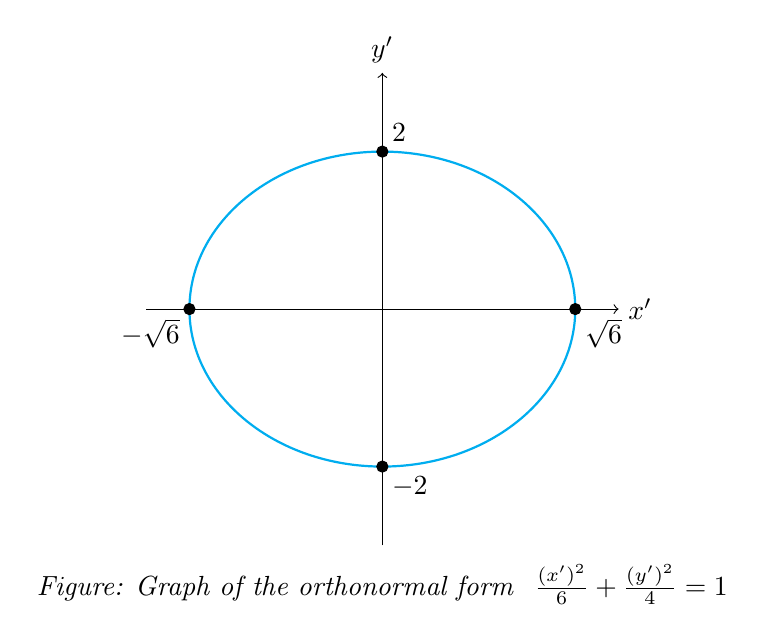
\begin{tikzpicture}
		% Draw Axes
		\draw[->] (-3,0) -- (3,0) node[right] {$x'$};
		\draw[->] (0,-3) -- (0,3) node[above] {$y'$};

		% Draw Ellipse
		\draw[thick, cyan] (0,0) ellipse (2.45cm and 2cm);

		% Label intercepts
		\filldraw (2.45,0) circle (2pt) node[anchor=north west] {$\sqrt{6}$};
		\filldraw (-2.45,0) circle (2pt) node[anchor=north east] {$-\sqrt{6}$};
		\filldraw (0,2) circle (2pt) node[anchor=south west] {$2$};
		\filldraw (0,-2) circle (2pt) node[anchor=north west] {$-2$};

		\node at (0,-3.5) {\textit{Figure: Graph of the orthonormal form } $\frac{(x')^2}{6} + \frac{(y')^2}{4} = 1$};
	\end{tikzpicture}
\end{center}

\pagebreak

% Question 16

\section{Question 16}
\textbf{Problem}
Determine whether the given matrix $A$ is diagonalizable. \\
If so, find the matrix $P$ that diagonalizes $A$ and the diagonal matrix $D$
such that $D = P^{-1}AP$.
\[
	A =
	\begin{bmatrix}
		1            & 2 \\
		-\frac{1}{2} & 1
	\end{bmatrix}
\]
\\
\\
\textbf{Solution}
\textbf{Step 1. Find Eigenvalues}
We find the eigenvalues by solving the characteristic equation
$\det(A - \lambda I) = 0$:
\begin{align*}
	\begin{vmatrix} 1 - \lambda & 2 \\ -1/2 & 1 - \lambda \end{vmatrix} & = 0 \\
	(1 - \lambda)(1 - \lambda) - (2)\left(-\frac{1}{2}\right)           & = 0 \\
	(1 - \lambda)^2 - (-1)                                              & = 0 \\
	(1 - \lambda)^2 + 1                                                 & = 0
\end{align*}
Solving for $\lambda$:
\begin{align*}
	(1 - \lambda)^2 & = -1            \\
	1 - \lambda     & = \pm \sqrt{-1} \\
	1 - \lambda     & = \pm i         \\
	\lambda         & = 1 \pm i
\end{align*}
The eigenvalues are $\lambda_1 = 1 + i$ and $\lambda_2 = 1 - i$.
\\
\\
\textbf{Conclusion}
Since the eigenvalues are complex (not real numbers), there are no corresponding
eigenvectors with real components. Therefore, the matrix $A$ is
\textit{not diagonalizable} over the field of real numbers $\mathbb{R}$.

\pagebreak

% Question 17

\section{Question 17}
\textbf{Problem}
If $\rho(x,y)$ is the density of a wire (mass per unit length), then
$m = \int_{C}{\rho(x,y)ds}$ is the mass of the wire.
\begin{enumerate}
    \item[i)] Find the mass of a wire having the shape of the semicircle $x=1+\cos t$, $y=\sin t$, $0 \le t \le \pi$, if the density at a point P is directly proportional to its distance from the y-axis.
    \item[ii)] Find the coordinates of the center of mass $(\bar{x}, \bar{y})$.
\end{enumerate}
\textbf{Solution}
\\
\\
\textbf{i) Find the Mass}
The mass is given by the line integral $m = \int_{C}{\rho(x,y)ds}$.
\\
\\
\textbf{1. Parameterization:}
\[
    \vec{r}(t) = (1 + \cos{t})\hat{i} + (\sin{t})\hat{j}, \quad 0 \le t \le \pi
\]
\\
\\
\textbf{2. Differential Element $ds$:}
Calculate the derivatives:
\[
    \frac{dx}{dt} = -\sin{t}, \quad \frac{dy}{dt} = \cos{t}
\]
Calculate the magnitude:
\[
    ds = \sqrt{\left(-\sin{t}\right)^{2} + \left(\cos{t}\right)^{2}} \, dt = \sqrt{\sin^{2}{t} + \cos^{2}{t}} \, dt = 1 \, dt
\]
\\
\\
\textbf{3. Density Function:}
The density is proportional to the distance from the y-axis ($|x|$). Since $x = 1 + \cos{t} \ge 0$ for the given domain:
\[
    \rho(x,y) = kx = k(1 + \cos{t})
\]
where $k$ is a constant of proportionality.
\\
\\
\textbf{4. Integral for Mass:}
\begin{align*}
    m &= \int_{0}^{\pi}{k(1 + \cos t)(1)dt}\\
      &= k \left[ t + \sin t \right]_{0}^{\pi} \\
      &= k [(\pi + 0) - (0 + 0)] \\
      &= k\pi
\end{align*}
\\
\\
\textbf{ii) Find Center of Mass}
The coordinates are given by $\bar{x} = M_{y}/m$ and
$\bar{y} = M_{x}/m$.
\\
\\
\textbf{Calculate $M_{y}$ (Moment about y-axis):}
\[
    M_{y} = \int_{C}{x \rho(x,y)ds} = \int_{0}^{\pi}{(1 + \cos{t}) k(1 + \cos{t})dt}
\]
\[
    M_{y} = k \int_{0}^{\pi}{(1 + \cos{t})^{2}dt} = k \int_{0}^{\pi}{(1 + 2\cos{t} + \cos^{2}{t})dt}
\]
Using the identity $\cos^{2}{t} = (1 + \cos{2t})/2$ :
\begin{align*}
    M_y &= k \int_{0}^{\pi}{\left( 1 + 2\cos{t} + \frac{1}{2} + \frac{1}{2}\cos{2t} \right)dt} \\
        &= k \int_{0}^{\pi}{\left( \frac{3}{2} + 2\cos{t} + \frac{1}{2}\cos{2t} \right)dt} \\
        &= k \left[\frac{3}{2}t + 2\sin{t} + \frac{1}{4}\sin{2t} \right]_{0}^{\pi} \\
        &= k \left[\left(\frac{3\pi}{2} + 0 + 0\right) - 0 \right] = \frac{3\pi k}{2}
\end{align*}
\[
    \bar{x} = \frac{M_y}{m} = \frac{3\pi k / 2}{k\pi} = \frac{3}{2}
\]
\\
\\
\textbf{Calculate $M_{x}$ (Moment about x-axis):}
\[
    M_{x} = \int_{C}{y \rho(x,y)ds} = \int_{0}^{\pi}{(\sin t) k(1 + \cos t)dt}
\]
\[
    M_{x} = k \int_{0}^{\pi}{(\sin t + \sin t \cos t)dt}
\]
Using simple integration for $\sin{t}$ and $u$-substitution (or identity
$\sin{2t}$) for $\sin{t} \cos{t}$:
\begin{align*}
    M_{x} &= k \left[ -\cos{t} + \frac{1}{2}\sin^{2}{t} \right]_{0}^{\pi} \\
        &= k \left[ (-\cos{\pi} + 0) - (-\cos{0} + 0) \right] \\
        &= k \left[ -(-1) - (-1) \right] = k(1 + 1) = 2k
\end{align*}
\[
    \bar{y} = \frac{M_{x}}{m} = \frac{2k}{k\pi} = \frac{2}{\pi}
\]
\\
\\
\textbf{Answer: }
The mass is $m = k\pi$, and the center of mass is located at
$\left(3/2, 2/\pi\right)$.

\pagebreak

% Question 18

\section{Question 18}
\textbf{Problem}
If $u = f(x,y)$ and $x = r\cos{\theta}, y = r\sin{\theta}$, show that Laplace's
Equation
\[

\]
\\
\\
\textbf{Solution}
\end{document}
